\documentclass[aspectratio=169]{beamer}
\title{Improvements and current status of the ACTS-based ITk main pass reconstruction}
\author{Andreas Stefl, Noemi Calace, Paul Gessinger-Befurt, Carlo Varni, Pierfrancesco Butti}
\institute{CERN}
\date{2025-08-18}

\setbeamertemplate{navigation symbols}{}

\begin{document}

\frame{\titlepage}

\begin{frame}
\frametitle{Abstract}
\tiny
The ATLAS experiment is carrying out an extensive upgrade effort for Phase-II of the LHC, including a new all-silicon Inner Tracker (ITk) [\href{https://cds.cern.ch/record/2257755}{ATLAS-TDR-025}, \href{https://cds.cern.ch/record/2285585}{ATLAS-TDR-030}]. One crucial part is a comprehensive software upgrade programme, whose goal is not only to achieve the ultimate physics performance, but at the same time to modernise the software technology, to make best use of upcoming and future processing technologies and ensure maintainability throughout the operation of the experiment. In order to achieve these objectives, the ATLAS Collaboration has decided to extensively use ACTS [\href{https://doi.org/10.1007/s41781-021-00078-8}{Ai X. et al., A Common Tracking Software Project, Comput Softw Big Sci 6, 8 (2022)}] for the Phase-II reconstruction software. ACTS is an experiment-independent toolkit for track reconstruction, which is designed from the ground up for thread-safety and high performance. It is built to accommodate different experiment deployment scenarios, and also serves as community platform for research and development of new approaches and algorithms in tracking. Using ACTS for ATLAS Phase-II reconstruction software allows us to directly profit from its thread-safety, high performance and code maintainability. Additionally, the migration to using ACTS also involves changes to the ATLAS Event-Data-Model [\href{https://cds.cern.ch/record/2014150}{ATL-SOFT-PROC-2015-003}] which, including adoption of the ACTS track representation, is interfaced with the ATLAS xAOD IO infrastructure [\href{https://cds.cern.ch/record/2767187}{ATL-SOFT-PUB-2021-001}].

In this contribution, the current status of the ACTS integration for the ATLAS ITk track reconstruction is presented; this builds on top of the previous status update [\href{https://cds.cern.ch/record/2921878}{ATL-SOFT-PROC-2025-012}]; when possible, physics and/or CPU performance comparisons with the none ACTS counterparts are presented. The performance of several algorithms in the track reconstruction chain is studied. The clusterization is the first step of event reconstruction: adjacent readout channels with a hit are grouped together in clusters for the ITk Pixel and Strip Detectors, respectively. A subsequent step produces space points, which are three-dimensional representations of clusters. Pixel and strip space points are used in the seeding stage of the track finding based on a combinatorial Kalman filter that is seeded from triplet space point combinations. For the efficiency and resolution plots, tracks are matched to true particles using a truth-matching probability of 50\%. This probability is defined as the ratio of the number of hits shared between a track and a particle and the total number of hits on the track. Pixel hits have a double relative weight with respect to strip measurements. All results are obtained using the ITk Layout 03-00-00 [\href{https://atlas.web.cern.ch/Atlas/GROUPS/PHYSICS/PLOTS/IDTR-2023-05}{IDTR-2023-05}].

Additionally, the ACTS \textit{Fast} configuration is included, which has been subject to a series of CPU time optimizations in the last months. This configuration is optimized for a potential high-level trigger application and modeled after the pre-existing Athena none ACTS \textit{Fast} configuration [\href{ATLAS-TDR-029-ADD-1}{https://cds.cern.ch/record/2802799}].
\end{frame}

\begin{frame}
\frametitle{Pixel clustering}
\begin{figure}[h]
    \centering
    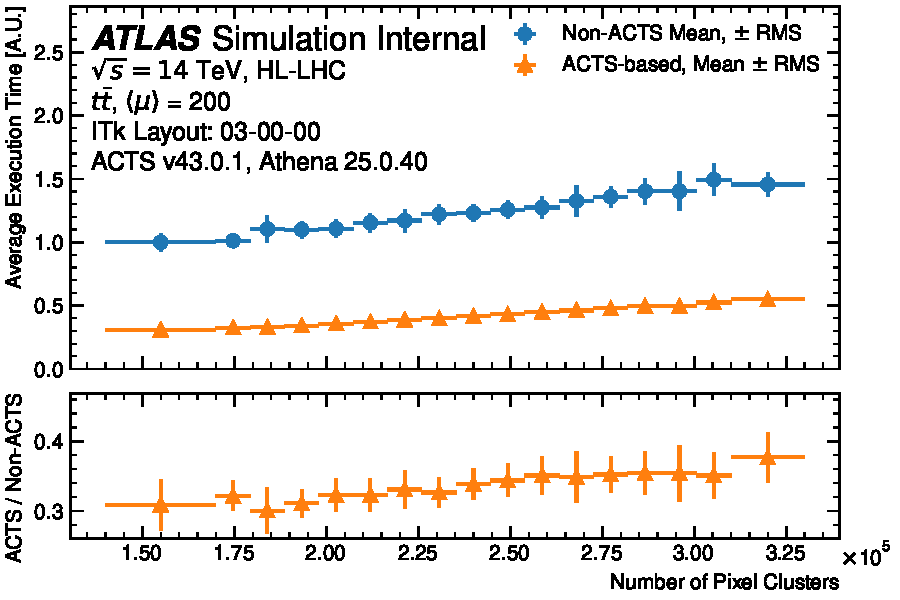
\includegraphics[width=0.8\textwidth]{plots/clustering_pixel.pdf}
\end{figure}
\end{frame}

\begin{frame}
\frametitle{Pixel clustering}
Average execution time (in arbitrary units) of the pixel clustering algorithms as a function of the number of reconstructed pixel clusters, obtained with the none ACTS implementation and an ACTS-based version. The measurement was taken on the same machine and the same set of $t\bar{t}$ events at $\langle \mu \rangle = 200$ with a center of mass energy of $\sqrt{s}=14$ TeV, using the ITk Layout 03-00-00. An average timing improvement per event of $\sim3\times$ with the ACTS-based version is observed while achieving identical physics results.
\end{frame}

\begin{frame}
\frametitle{Strip clustering}
\begin{figure}[h]
    \centering
    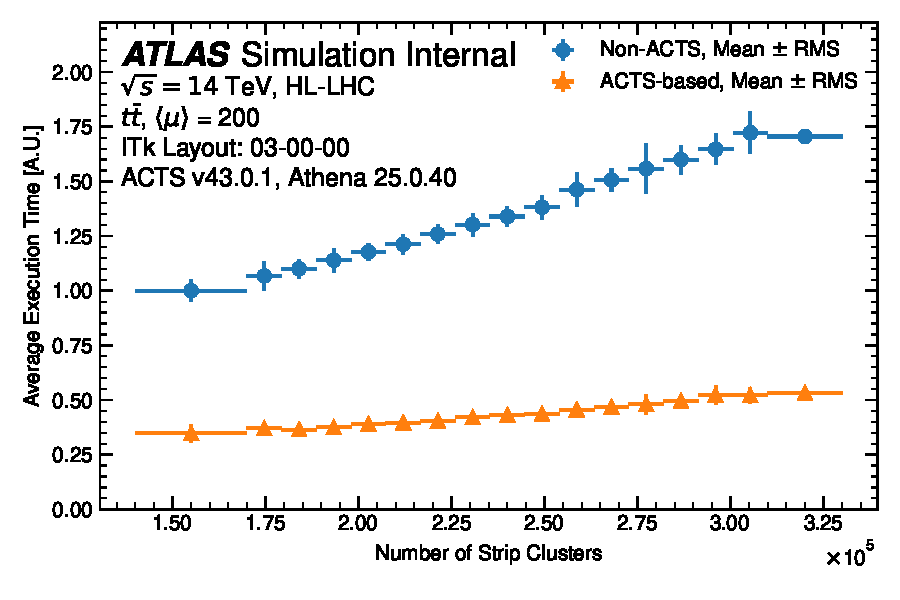
\includegraphics[width=0.8\textwidth]{plots/clustering_strip.pdf}
\end{figure}
\end{frame}

\begin{frame}
\frametitle{Strip clustering}
Average execution time (in arbitrary units) of the strip clustering algorithms as a function of the number of reconstructed strip clusters, obtained with the none ACTS implementation and an ACTS-based version. The measurement was taken on the same machine and the same set of $t\bar{t}$ events at $\langle \mu \rangle = 200$ with a center of mass energy of $\sqrt{s}=14$ TeV, using the ITk Layout 03-00-00. An average timing improvement per event of $\sim3\times$ with the ACTS-based version is observed while achieving identical physics results.
\end{frame}

% \begin{frame}
% \frametitle{Pixel seeding}
% \begin{figure}[h]
%     \centering
%     \includegraphics[width=0.8\textwidth]{plots/seeding_pixel.pdf}
% \end{figure}
% \end{frame}

\begin{frame}
\frametitle{Tracking efficiency}
\begin{figure}[h]
    \centering
    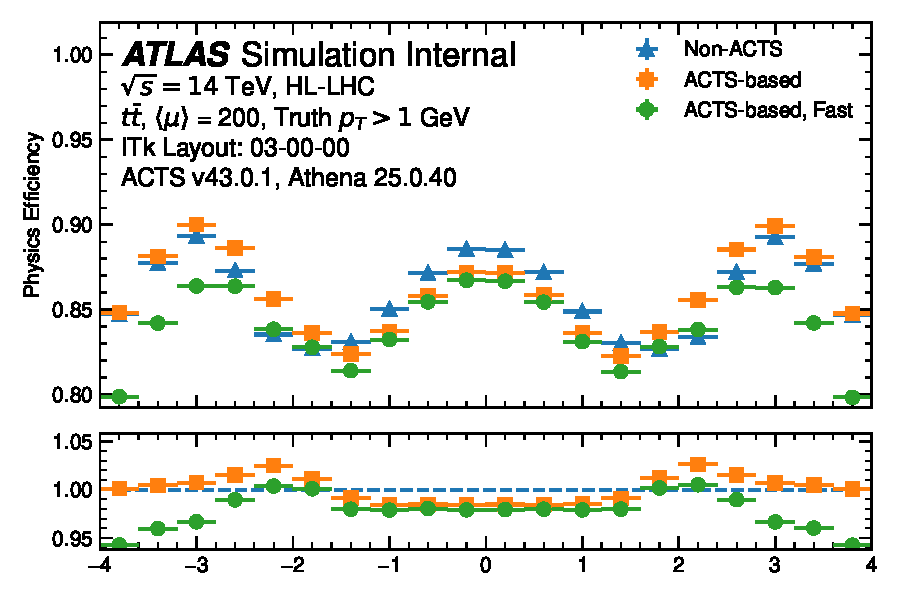
\includegraphics[width=0.8\textwidth]{plots/tracking_efficiency_physics.pdf}
\end{figure}
\end{frame}

\begin{frame}
\frametitle{Tracking efficiency}
Tracking efficiency as a function of the pseudo-rapidity $\eta$ of the associated truth particle using the ITk Layout 03-00-00 for $t\bar{t}$ events at $\langle \mu \rangle = 200$. ACTS-based chains are compared to the none ACTS implementation. Lower efficiency is observed in the barrel region $|\eta| < 1.5$. The ACTS-based fast configuration drops further in the endcap region $|\eta| > 2.0$ which is due to CPU optimization trade-offs and under investigation.
\end{frame}

\begin{frame}
\frametitle{Tracking resolution $\sigma(d_0)$}
\begin{figure}[h]
    \centering
    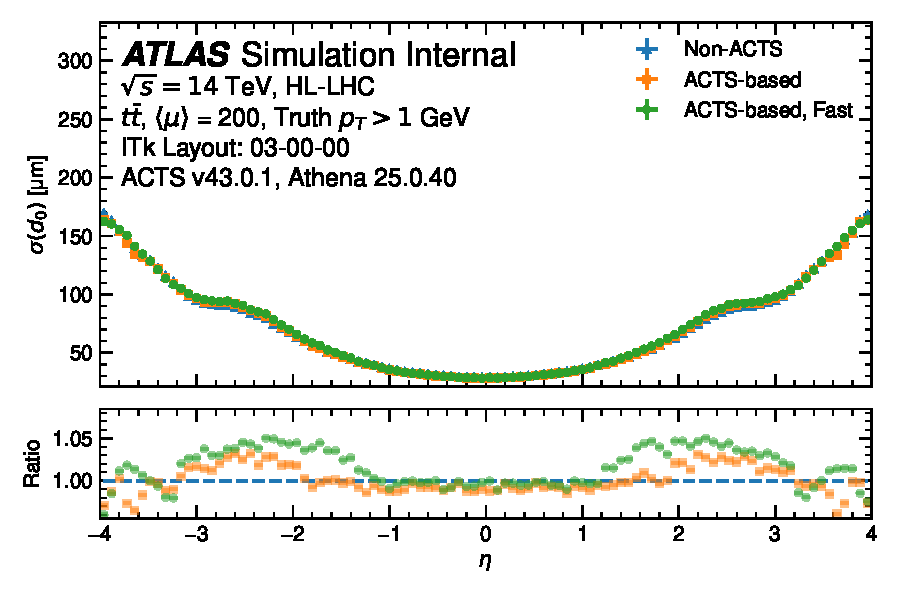
\includegraphics[width=0.8\textwidth]{plots/tracking_resolution_d0.pdf}
\end{figure}
\end{frame}

\begin{frame}
\frametitle{Tracking resolution $\sigma(d_0)$}
Transverse impact parameter $d_0$ resolution as a function of the pseudo-rapidity $\eta$ of the associated truth particle using the ITk Layout 03-00-00 for $t\bar{t}$ events at $\langle \mu \rangle = 200$.
\end{frame}

\begin{frame}
\frametitle{Tracking resolution $\sigma(z_0)$}
\begin{figure}[h]
    \centering
    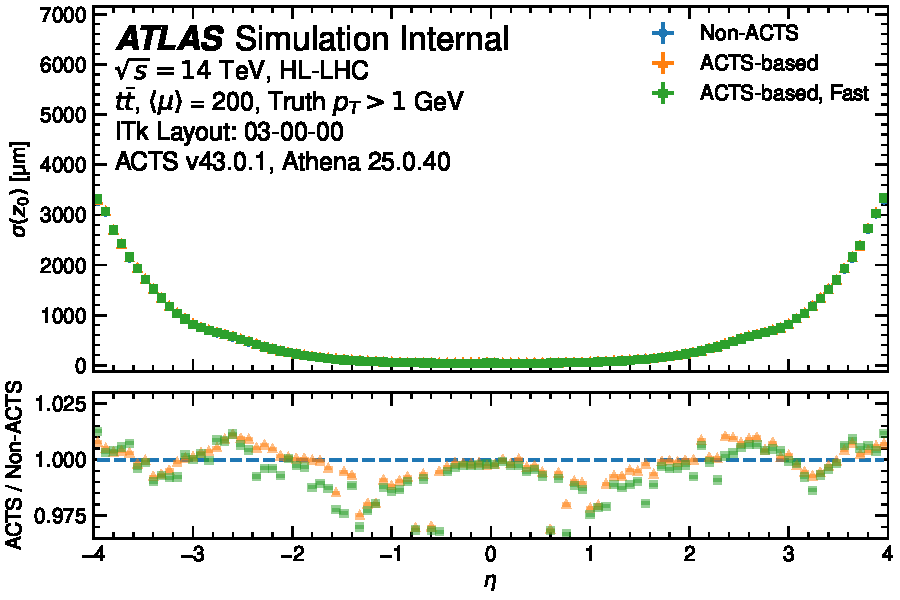
\includegraphics[width=0.8\textwidth]{plots/tracking_resolution_z0.pdf}
\end{figure}
\end{frame}

\begin{frame}
\frametitle{Tracking resolution $\sigma(z_0)$}
Longitudinal impact parameter $z_0$ resolution as a function of the pseudo-rapidity $\eta$ of the associated truth particle using the ITk Layout 03-00-00 for $t\bar{t}$ events at $\langle \mu \rangle = 200$.
\end{frame}

\begin{frame}
\frametitle{Tracking resolution $p_T \ \sigma(q/p_T)$}
\begin{figure}[h]
    \centering
    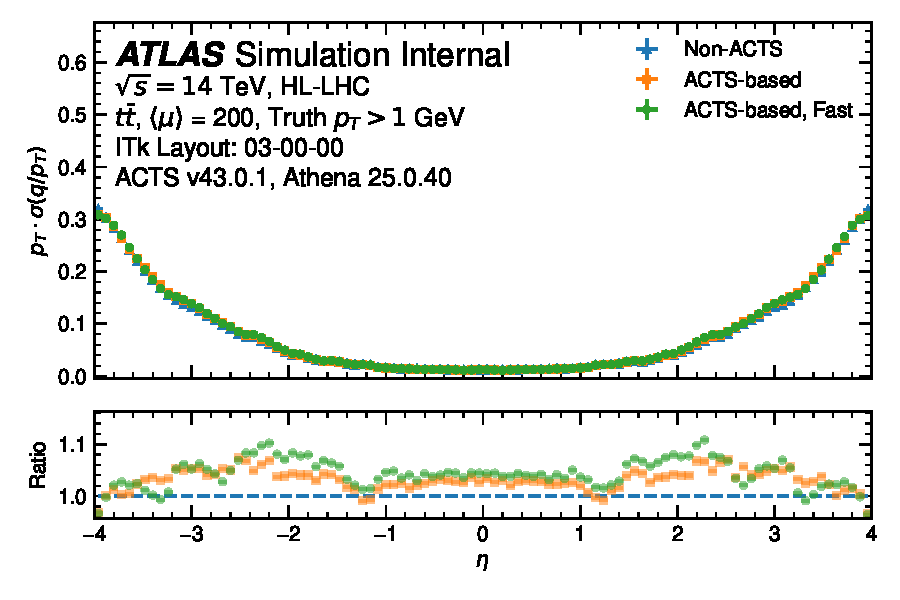
\includegraphics[width=0.8\textwidth]{plots/tracking_resolution_ptqopt.pdf}
\end{figure}
\end{frame}

\begin{frame}
\frametitle{Tracking resolution $p_T \ \sigma(q/p_T)$}
Relative transverse momentum $p_T$ resolution as a function of the pseudo-rapidity $\eta$ of the associated truth particle using the ITk Layout 03-00-00 for $t\bar{t}$ events at $\langle \mu \rangle = 200$.
\end{frame}

\begin{frame}
\frametitle{CPU time evolution}
\begin{figure}[h]
    \centering
    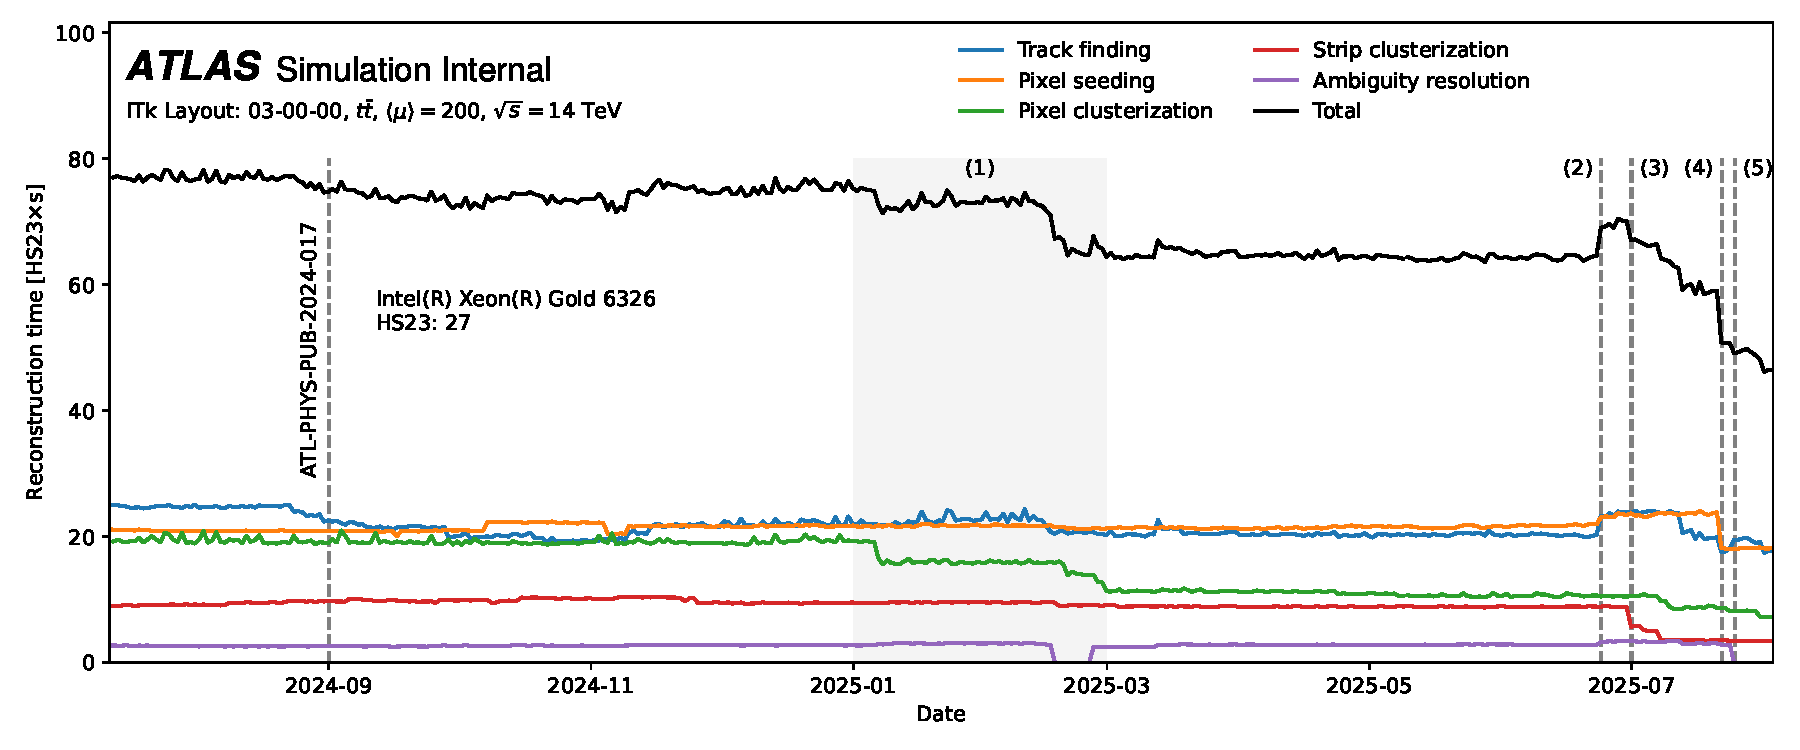
\includegraphics[width=1.0\textwidth]{plots/spot.pdf}
\end{figure}
\end{frame}

\begin{frame}
\frametitle{CPU time evolution}
CPU time evolution of the ACTS-based ITk main pass reconstruction, \textit{Fast} configuration, measured on a single core of a Intel Xeon Gold 6148. All measurements were taken on the same machine and the same set of $t\bar{t}$ events at $\langle \mu \rangle = 200$ with a center of mass energy of $\sqrt{s}=14$ TeV, using the ITk Layout 03-00-00. The measured reconstruction time is scaled to HS23$\times$s. On a high level, the major changes include: (1) series of optimizations on the pixel clustering, (2) lowering the $p_T$ reconstruction cut from 1 GeV to 900 MeV, (3) optimization of the strip clustering, (4) tuning the redundancy of the pixel seeding, (5) merging the ambiguity resolution into the track finding.
\end{frame}

\end{document}
